\section{Resultados Obtenidos}

\begin{frame}{Resultados Obtenidos}
\framesubtitle{Metodolog\'ia}

\begin{table}[H]
\centering
\footnotesize
\caption{Resumen de las variables de la prueba de usabilidad}
\begin{tabular}{|p{1.2cm}|p{2.4cm}|}
\hline
Factor  &   Promedio \\
\hline
$A$  &      83,70 \%     \\
$E_1$ &     16,30 \%  \\
$E_2$  &    5,91  \%  \\
$T_{1+2}$ & 13,83  minutos  \\
$T_{3+4}$ & 18,35  minutos  \\
$E_3$ &     11,83  errores  \\
$C$ &       87,5   \%  \\
$M$ &       12,75  palabras  \\
$U$ &       40.67  comandos  \\
\hline  
\end{tabular}
\label{sec:tabla-resumen-prueba}
\end{table}

\end{frame}

\begin{frame}{Resulados Obtenidos}
\framesubtitle{Correlaci\'on}
\begin{table}[H] 
\centering
\footnotesize
\begin{tabular}{|p{0.7cm}|p{0.7cm}|p{0.7cm}|p{0.7cm}|p{0.7cm}|p{0.7cm}|p{0.7cm}|p{0.7cm}|p{0.7cm}|p{0.7cm}|}
\hline
& $M$ &  $A$  &   $E_1$ &  $E_2$  &  $T_{1+2}$  & $T_{3+4}$     & $E_3$ & $C$ & $U$ \\
\hline
$M$       &  1     &  0,22  & -0,22  & -0,38  &  -0,31  &  -0,42  &  -0,29 & -0,08    &  -0,23 \\
$A$       &  0,22  &  1  &  -1  &  0,51  &  0,14  &  -0,09  &  0,69  &  0,5           &  0,53 \\
$E_1$     &  -0,22 &  -1  &  1  &  -0,51  &  -0,14  &  0,09  &  -0,69  &  -0,5        &  -0,53 \\
$E_2$     &  -0,38 &  0,51  &  -0,51  &  1  &  0,4  &  0,23  &  0,71  &  0,29         &  0,35  \\
$T_{1+2}$ &  -0,31 &  0,14  &  -0,14  &  0,4  &  1  &  0,87  &  0,57  &  -0,04        &  0,25 \\
$T_{3+4}$ &  -0,42 &  -0,09  &  0,09  &  0,23  &  0,87  &  1  &  0,37  &  -0,16       &  0,2 \\
$E_3$     &  -0,29 &  0,69  &  -0,69  &  0,71  &  0,57  &  0,37  &  1  &  0,28        &  0,52 \\
$C$       &  -0,08 &  0,5  &  -0,5  &  0,29  &  -0,04  &  -0,16  &  0,28  &  1        &  0,13 \\
$U$       &  -0,23 &  0,53  &  -0,53  &  0,35  &  0,25  &  0,2  &  0,52  &  0,13      &  1 \\
\hline
\end{tabular}
\caption{Coeficientes de correlaci\'on para las m\'etricas consideradas.}
\label{sec:tabla-correlacion}
\end{table}

\end{frame}

\begin{frame}{Resultados Obtenidos}
\framesubtitle{An\'alisis del Error Humano}
\begin{table}[H]
\centering
\footnotesize
\begin{tabular}{|p{1.2cm}|p{1.0cm}|p{1.0cm}|p{1.0cm}|p{1.0cm}|p{1.0cm}|}
\hline
    Sujeto & 2 & 3 & 4 & 5 & 6  \\
    \hline 
    Promedio & 6,96 & 5,68 & 7,46 & 14,81 & 42,11 \\
\hline
\end{tabular}
\caption{Tasa de error humano por longitud del comando.}
\label{sec:error-longitud}
\end{table}


\begin{table}[H]
\centering
\footnotesize
\begin{tabular}{|p{1.6cm}|p{1.6cm}|p{1.6cm}|p{1.6cm}|}
\hline
    Sujeto & General & Pista & Comp\'as \\
\hline
Promedio & 13,25 & 3,57 & 5,16 \\
\hline
\end{tabular}
\caption{Tasa de error humano por nivel contextual del comando.}
\label{sec:error-contexto}
\end{table}


\begin{table}[H]
\centering
\footnotesize
\begin{tabular}{|l|p{3cm}|}
\hline
Comando & Tasa de Error \\
\hline
crear nueva partitura & 18,38 \\
duplicar pista uno en pista dos & 17,5 \\
duplicar pista uno en pista tres & 16,67 \\
duplicar pista tres en pista cuatro & 13,25 \\
comp\'as cuatro & 13,19 \\
\hline
\end{tabular}
\caption{Lista de comandos con mayor tasa de error humano promedio.}
\label{sec:tabla-lista-comandos-error}
\end{table}


\end{frame}


\begin{frame}{Resultados Obtenidos}
\framesubtitle{An\'alisis del Error Humano}

\begin{columns}
\column{0.35\linewidth}
\centering
\begin{table}
\tiny
\begin{tabular}{|c|c|}
\hline
    Etapa & \% de la Tasa de Error Total \\
    \hline
0-10  &  11,62 \\
10-20 &  13.49 \\
20-30 &  12,29 \\
30-40 &  17,78 \\
40-50 &  6,85 \\
50-60 &  3,75 \\
60-70 &  9,92 \\
70-80 &  2,76 \\
80-90 &  12,12 \\
90-100 & 9,42 \\
    \hline
\end{tabular}
\caption{Distribuci\'on del error humano por etapas de la sesi\'on.}
\label{sec:error-tiempo}
\end{table}

\column{0.65\linewidth}
\begin{figure}
\centering
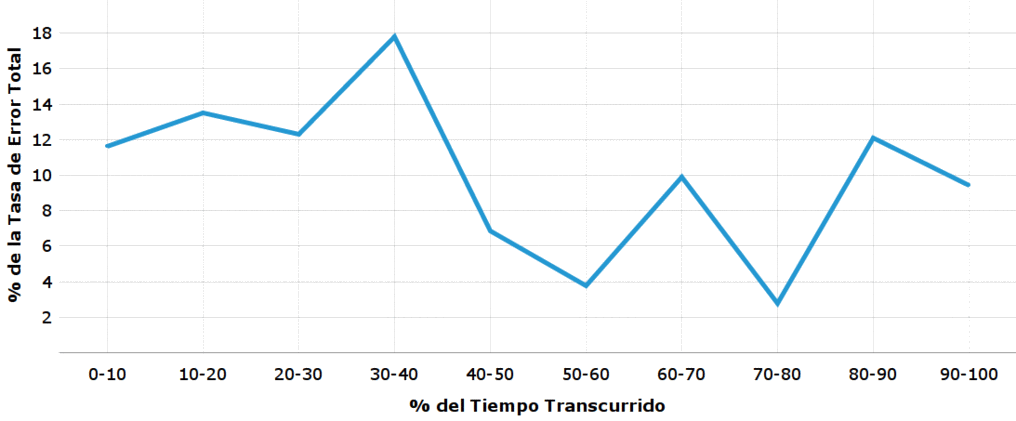
\includegraphics[width=1\linewidth]{./graphics/error_tiempo.png}
\caption{Distribuci\'on del error humano por etapas de la sesi\'on.}
\label{figure:gerror-tiempo}
\end{figure}
\end{columns}

\end{frame}

\begin{frame}{Resultados Obtenidos}
\framesubtitle{Encuesta}
\begin{columns}
\column{0.35\linewidth}
\begin{table}[H] 
\centering
\tiny
\begin{tabular}{|r|r|r|r|r|}
\hline
            & Promedio \\
\hline
Palabras    & 6.17 \\
Comandos    & 6.58 \\
Entrenamiento  & 6.25 \\
Interfaz por Voz & 5.83 \\
\hline
\end{tabular}
\caption{Resumen de la encuesta realizada.}
\label{sec:tabla-encuesta}
\end{table}
\column{0.65\linewidth}
\begin{figure}[ht]
\centering
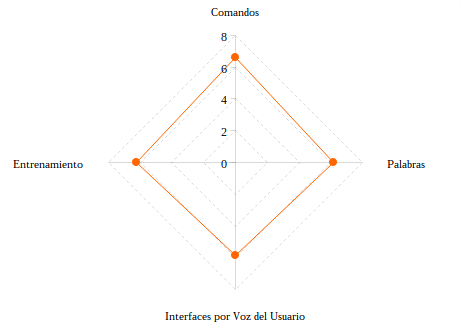
\includegraphics[width=1\linewidth]{./graphics/kiviat0.png}
\caption{Gr\'afico radial resumen de la encuesta realizada.}
\label{figure:kiviat-encuesta1}
\end{figure}
\end{columns}
\end{frame}

\begin{frame}{Resultados Obtenidos}
\framesubtitle{Encuesta}
\begin{columns}
\column{0.35\linewidth}
\begin{table}[H] 
\centering
\tiny
\begin{tabular}{|r|r|r|r|r|}
\hline
            & Promedio \\
\hline
Palabras    & 0.45 \\
Comandos    & 0.86 \\
Entrenamiento  & 0.55 \\
Interfaz por Voz & 0.5 \\
\hline
\end{tabular}
\caption{Resumen de la encuesta realizada. Valores reescalados.}
\label{sec:tabla-encuesta-normalizada}
\end{table}
\column{0.65\linewidth}
\begin{figure}[ht]
\centering
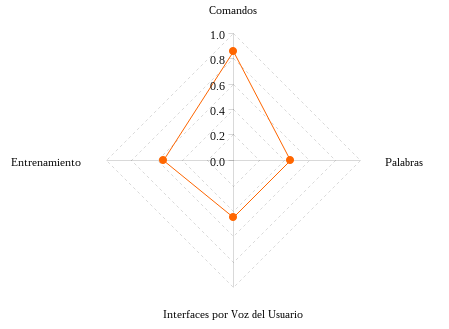
\includegraphics[width=1\linewidth]{./graphics/kiviat.png}
\caption{Gr\'afico radial resumen de la encuesta realizada. Valores reescalados.}
\label{figure:kiviat-encuesta2}
\end{figure}
\end{columns}
\end{frame}